\section{Introduction to Deep Learning and PyTorch}\label{sec:deep-learning}

\subsection{Neural Networks and Deep Learning}\label{sec:dl-nn}

\textit{Fully connected Neural Networks} are stacks of linear functions and nonlinear activation functions; they have much more representational power than linear classifiers. This kind of neural network is also called \textit{multi-layer perceptrons}.

While in linear classifier (such as the SVM) we had the linear score function $f = Wx$ (see \ref{eq:linear-classifier}), with a 2-layers NN we use the function
\begin{equation}\label{eq:2-mlp}
f = W_2 \max(0, W_1 x)
\end{equation}
with $x \in \mathbb{R}^D, W_1 \in \mathbb{R}^{H \times D}, W_2 \in \mathbb{R}^{C \times H}$, similarly, with a 3-layers NN we use
\begin{equation}\label{eq:3-mlp}
f = W_3 \max(0, W_2 \max(0, W_1 x))
\end{equation}
with $x \in \mathbb{R}^D, W_1 \in \mathbb{R}^{H \times D}, W_2 \in \mathbb{R}^{C \times H}$ (see figure \ref{fig:3mlp}).\\
Note that in practice we usually add a learnable \textit{bias} at each layer as well.

\begin{figure}[!h]
    \centering
    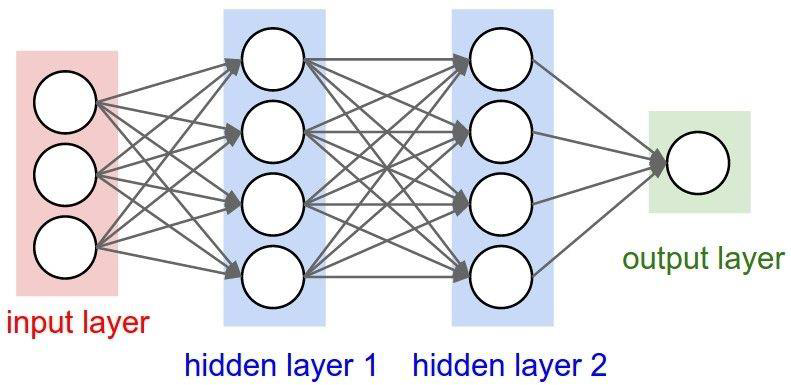
\includegraphics[width=0.7\linewidth]{3mlp}
    \caption[3-layer Neural Network]{3-layer Neural Network}
    \label{fig:3mlp}
\end{figure}

The non linear function $\max(0,z)$ is an \textbf{activation function}. Note that without using it we end up with a new linear classifies, that isn't useful at all.

Some (non linear) activation functions that may be used are: \label{dl-activation}
\begin{myitem}
    \item ReLU: $\max(0,x)$,
    \item Sigmoid: $\sigma(x) = \frac{1}{1 + e^{-x}}$,
    \item Tanh: $\tanh(x)$,
    \item Leaky ReLu: $\max(0.1x,x)$,
    \item Maxout: $\max(W_1^T x + b_1, W_2^T x + b_2)$,
    \item ELU:
    $\begin{cases}
    x              &x \geq 0\\
    \alpha(e^x -1) &x < 0
    \end{cases}$.
\end{myitem}

It's important to note that increasing the number of layers and their size (the number of neurons per layer) leads to an improvement to the capacity of the NN, but increases overfitting too: the network adapts too well to the input data, so it isn't able to generalize (see figure \ref{fig:dl-overfitting}). Thus, we use regularization to solve this problem (see figure \ref{fig:dl-regularization}).

\begin{minipage}{.5\linewidth}
    \begin{figure}[H]
        \centering
        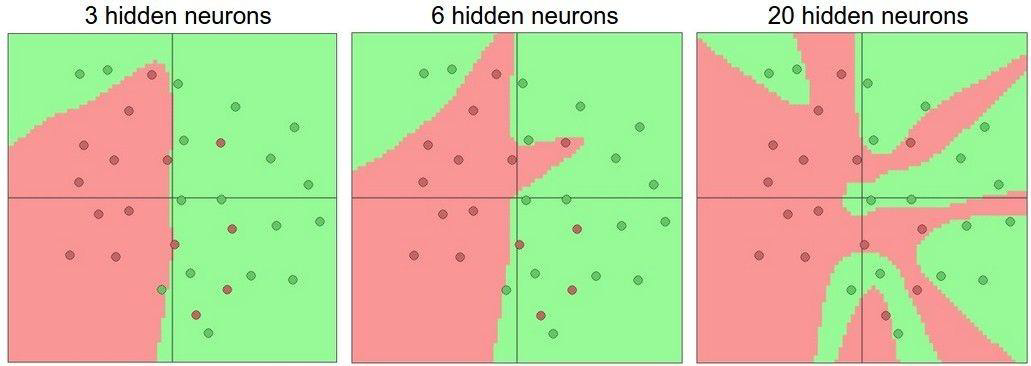
\includegraphics[width=0.9\linewidth]{nn-overfitting}
        \caption[The effect of increasing the number of neurons]{The effect of increasing the\\ number of neurons}
        \label{fig:dl-overfitting}
    \end{figure}
\end{minipage}
\begin{minipage}{.5\linewidth}
    \begin{figure}[H]
        \centering
        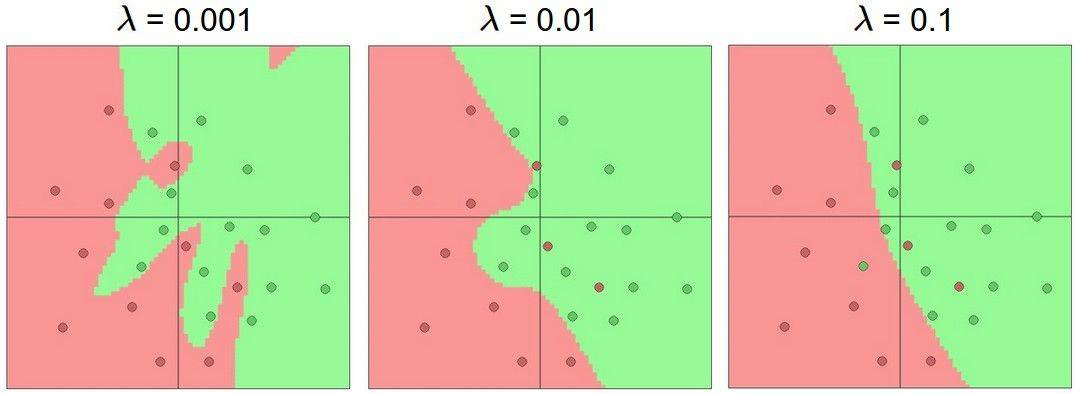
\includegraphics[width=0.9\linewidth]{nn-regularization}
        \caption[The effect of increasing the regularization's strength]{The effect of increasing the\\ regularization's strength}
        \label{fig:dl-regularization}
    \end{figure}
\end{minipage}

While it is possible to compare the artificial neurons with the biological ones, since they receive electrical stimuli from other synapses through dendrites, and propagates the impulse according to a sort of activation function of the received stimuli, like the one computed in NNs, there are some important differences between them:
\begin{myitem}
    \item Biological neurons have complex connectivity patterns, while artificial ones are organized into regular layers for computational efficiency (even if NN with random connections can work too);
    \item There exists many different types of biological neurons;
    \item Dendrites can perform complex non linear computations;
    \item Synapses are not a single weight but a complex non linear dynamical system;
    \item Rate code may not be adequate.
\end{myitem}

Since, as we saw, the number of layers of the network (\textit{depth}) increases its capacity, we are particularly interest in \textbf{Deep Neural Networks}, that is, those networks with many hidden layers.

\begin{figure}[h!]
    \centering
    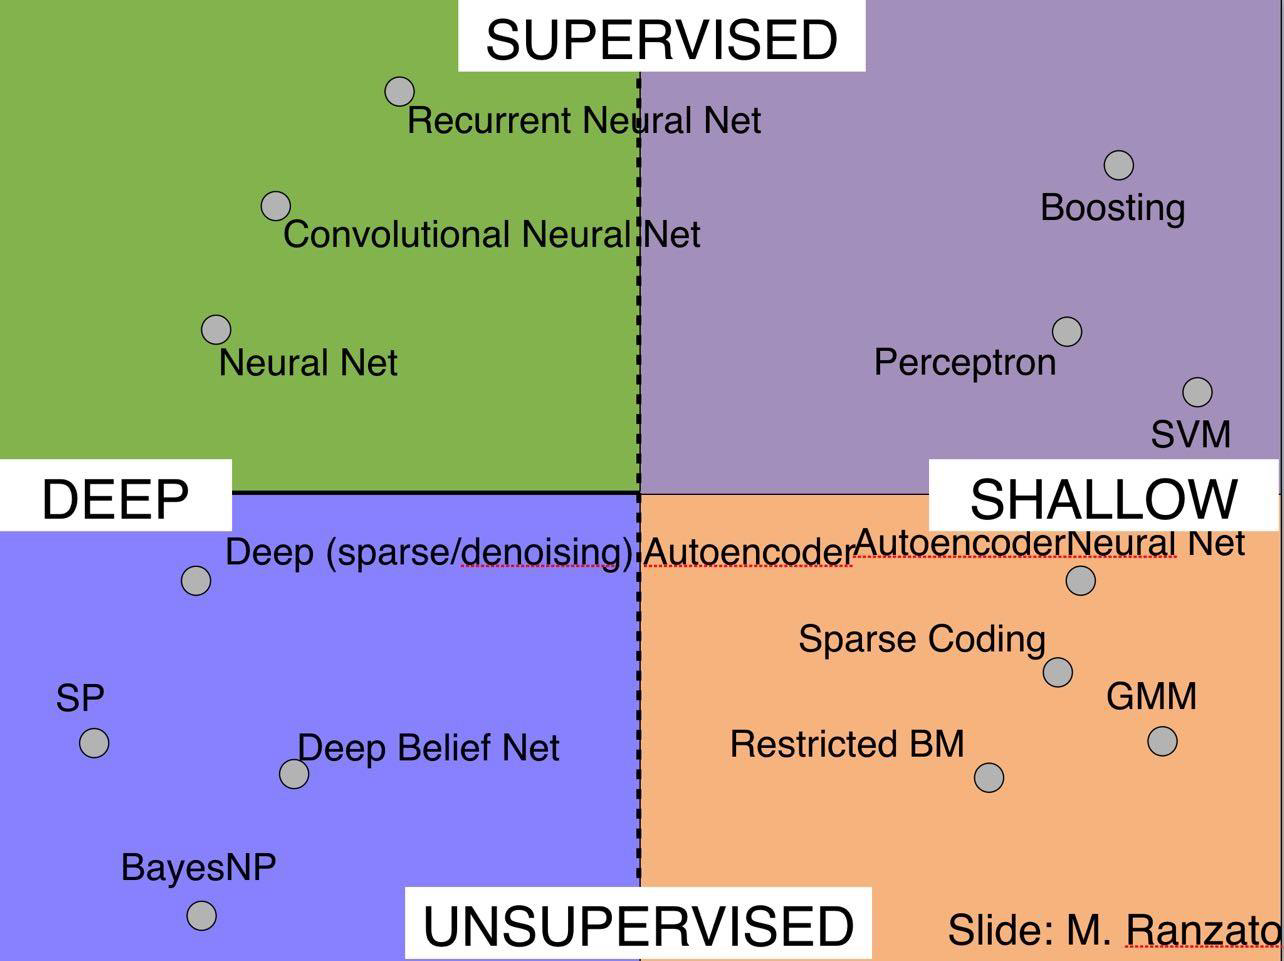
\includegraphics[width=0.6\linewidth]{nn-architectures}
    \caption[Overview of Neural Network Architectures]{Overview of Neural Network Architectures}
    \label{fig:dl-architectures}
\end{figure}

Deep Learning is giving so good result and performances thanks to different factors:
\begin{myitem}
    \item Availability of large datasets;
    \item Massive parallel compute power;
    \item Advances in machine learning over the years;
    \item Internet (availability of large scale data);
    \item GPUs (availability of parallel compute power);
    \item Deep / hierarchical models with end to end learning.
\end{myitem}

Thanks to the progress of deep networks, the process of feature extraction we sketched in section \ref{sec:ic-image-features} has changed dramatically. The traditional approach is:
\begin{myitem}
    \item features are hand crafted and fixed,
    \item extracted features might be too general or too specific,
    \item to achieve best classification performance more complex classifier are built.
\end{myitem}
The research on hand-crafted features lead to considerable improvements over the years, and many hand designed features are currently in use.

With deep learning, though, we can perform parameterized feature extraction, and we can obtain features that are efficient to compute and to train (differentiable), by joining the training of feature extraction and of classification into one pipeline, a \textit{unique end-to-end system}. In this way, all parts are adaptive, and we can apply a nonlinear transformation directly from input to desired output. Furthermore, we can built complex networks just by composition of simple building blocks: each block has its trainable parameters and produces an intermediate representation of the input image, more abstract from layer to layer. Like in MLP, during the forward pass the output is generated, than the error is propagated backwards to update weights in the backpropagation step.


\subsection{Deep Learning Hardware}\label{sec:dl-hw}

CPUs and GPUs are the most important hardware for Deep Learning. Let's see the differences between them:
\begin{myitem}
    \item \textbf{CPU}:
    \begin{myitem}
        \item Fewer cores, but each core is much faster and much more capable,
        \item Great at sequential tasks;
    \end{myitem}
    \item \textbf{GPU}:
    \begin{myitem}
        \item More cores, but each core is much slower and “dumber”,
        \item Great for parallel tasks;
    \end{myitem}
    \item \textbf{TPU}: New hardware specialized for deep learning, by Google.
\end{myitem}
Note that NVIDIA GPUs are more supported than AMD ones in machine learning frameworks such as TensorFlow or PyTorch, thanks to the \textit{CUDA Deep Neural Network} library.

\begin{minipage}{.5\linewidth}
    \begin{figure}[H]
        \centering
        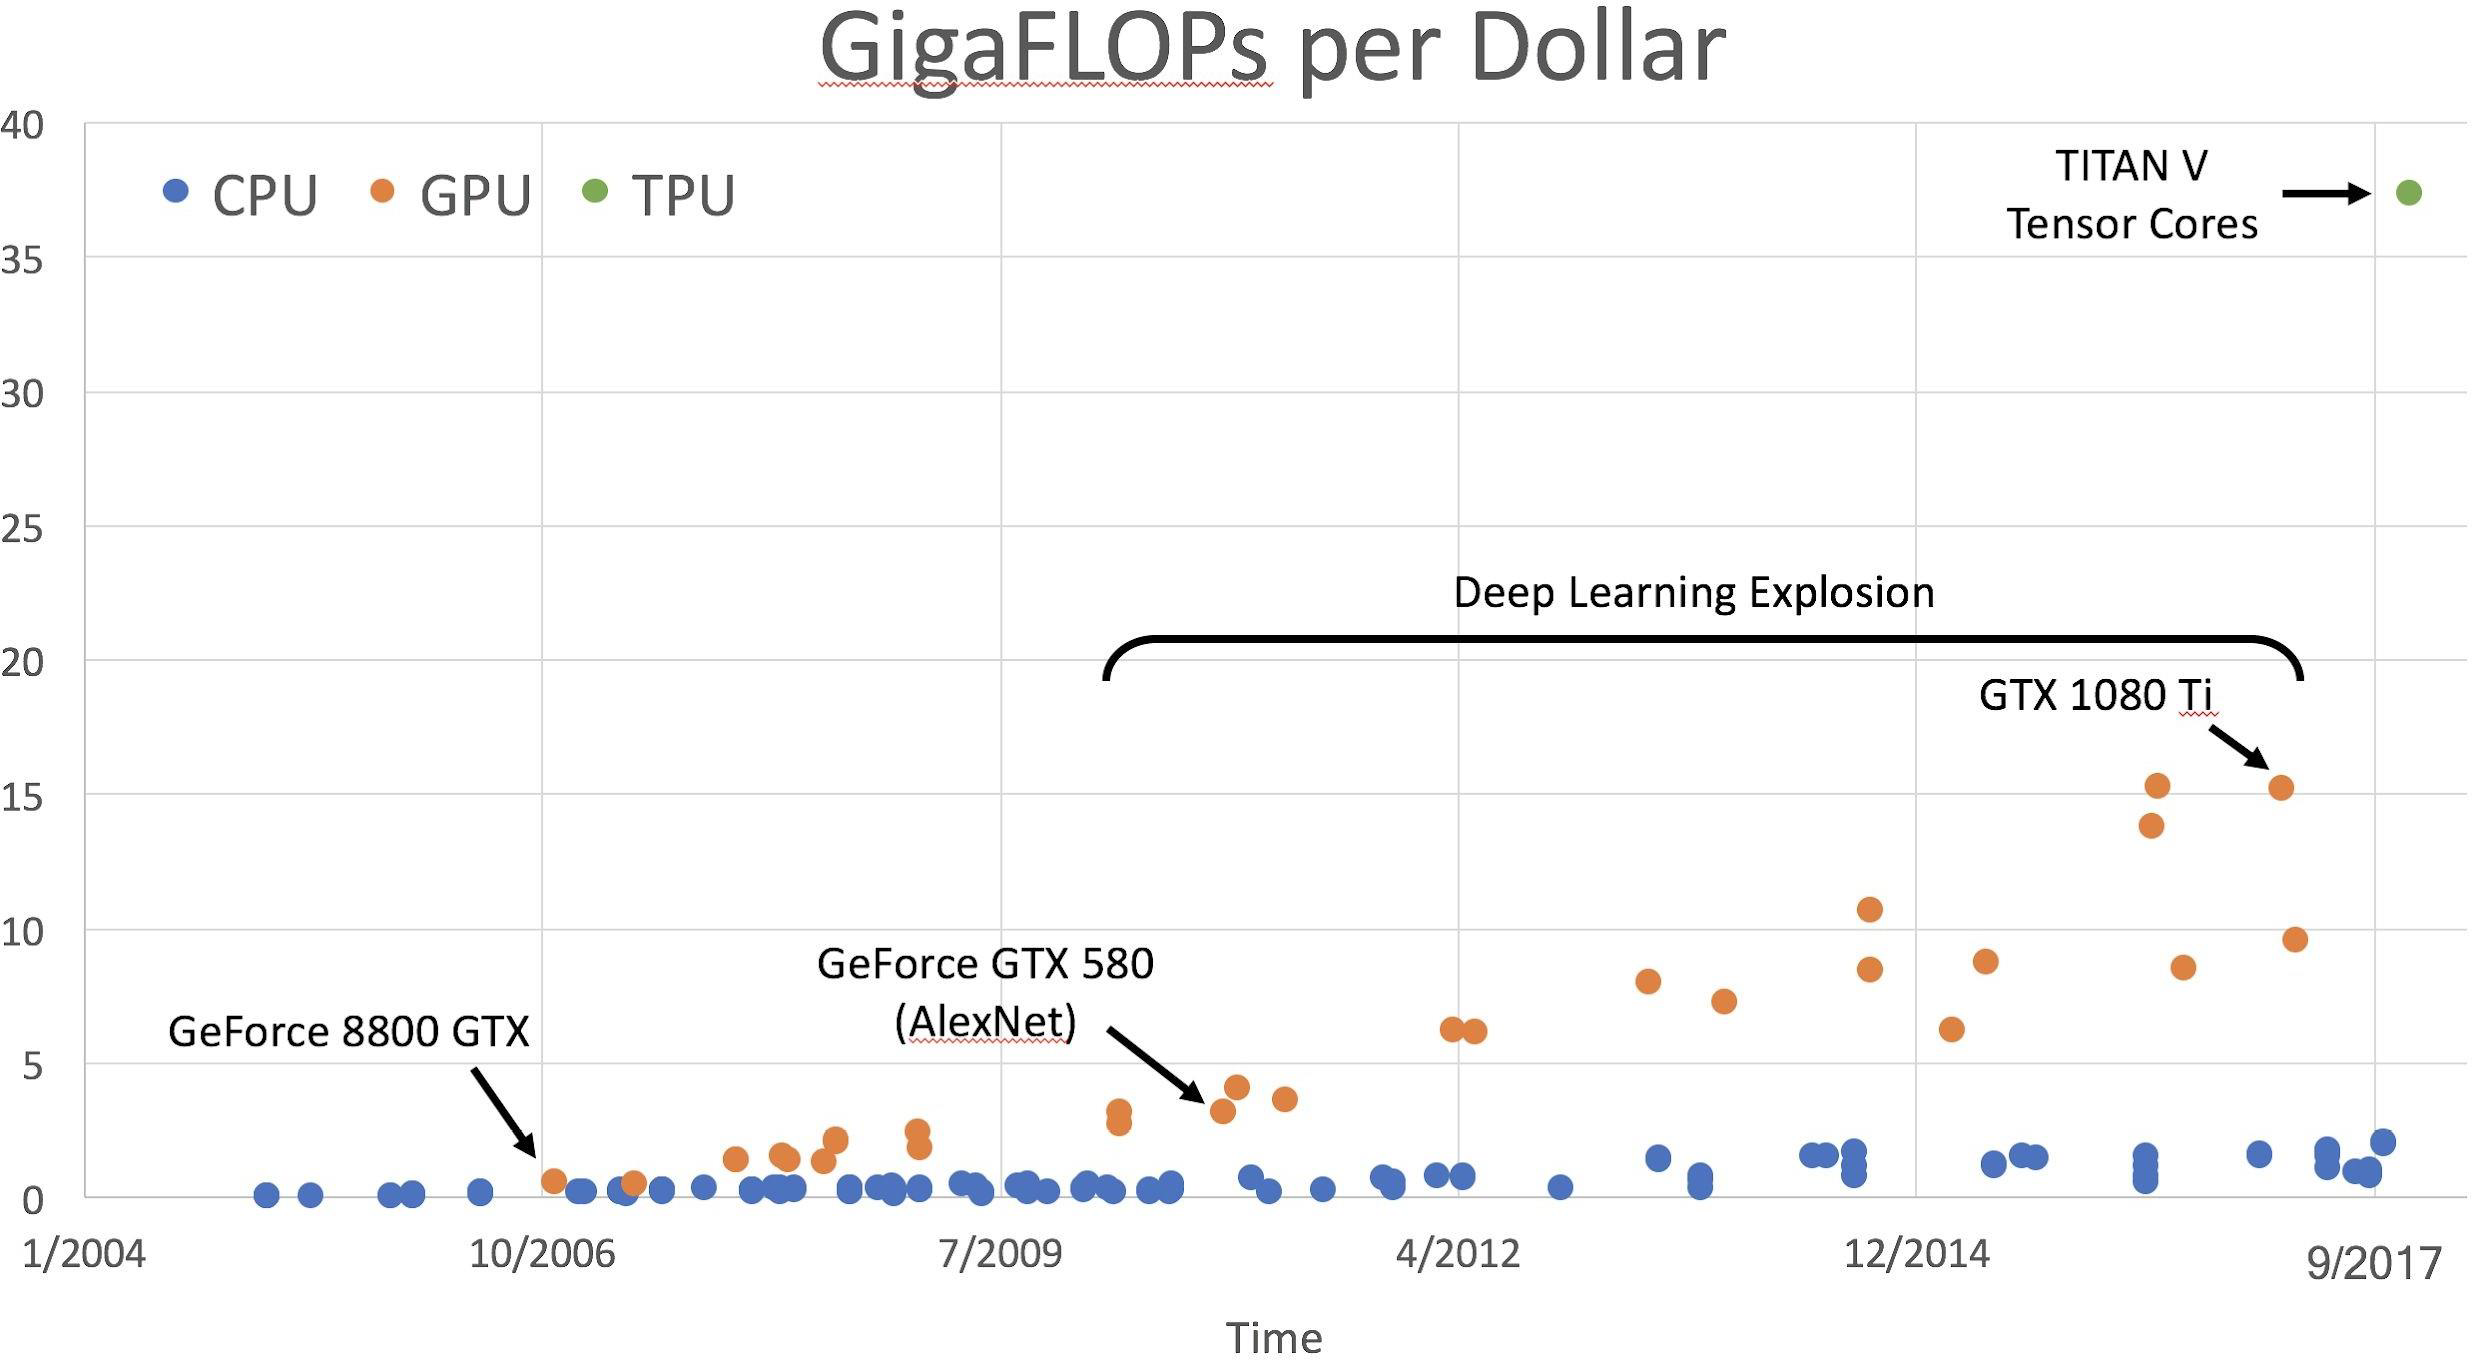
\includegraphics[width=0.9\linewidth]{images/dl-gpus1}
        \caption[The evolution of CPUs adn GPUs]{The evolution of CPUs adn GPUs}
        \label{fig:dl-gpus1}
    \end{figure}
\end{minipage}
\begin{minipage}{.5\linewidth}
    \begin{figure}[H]
        \centering
        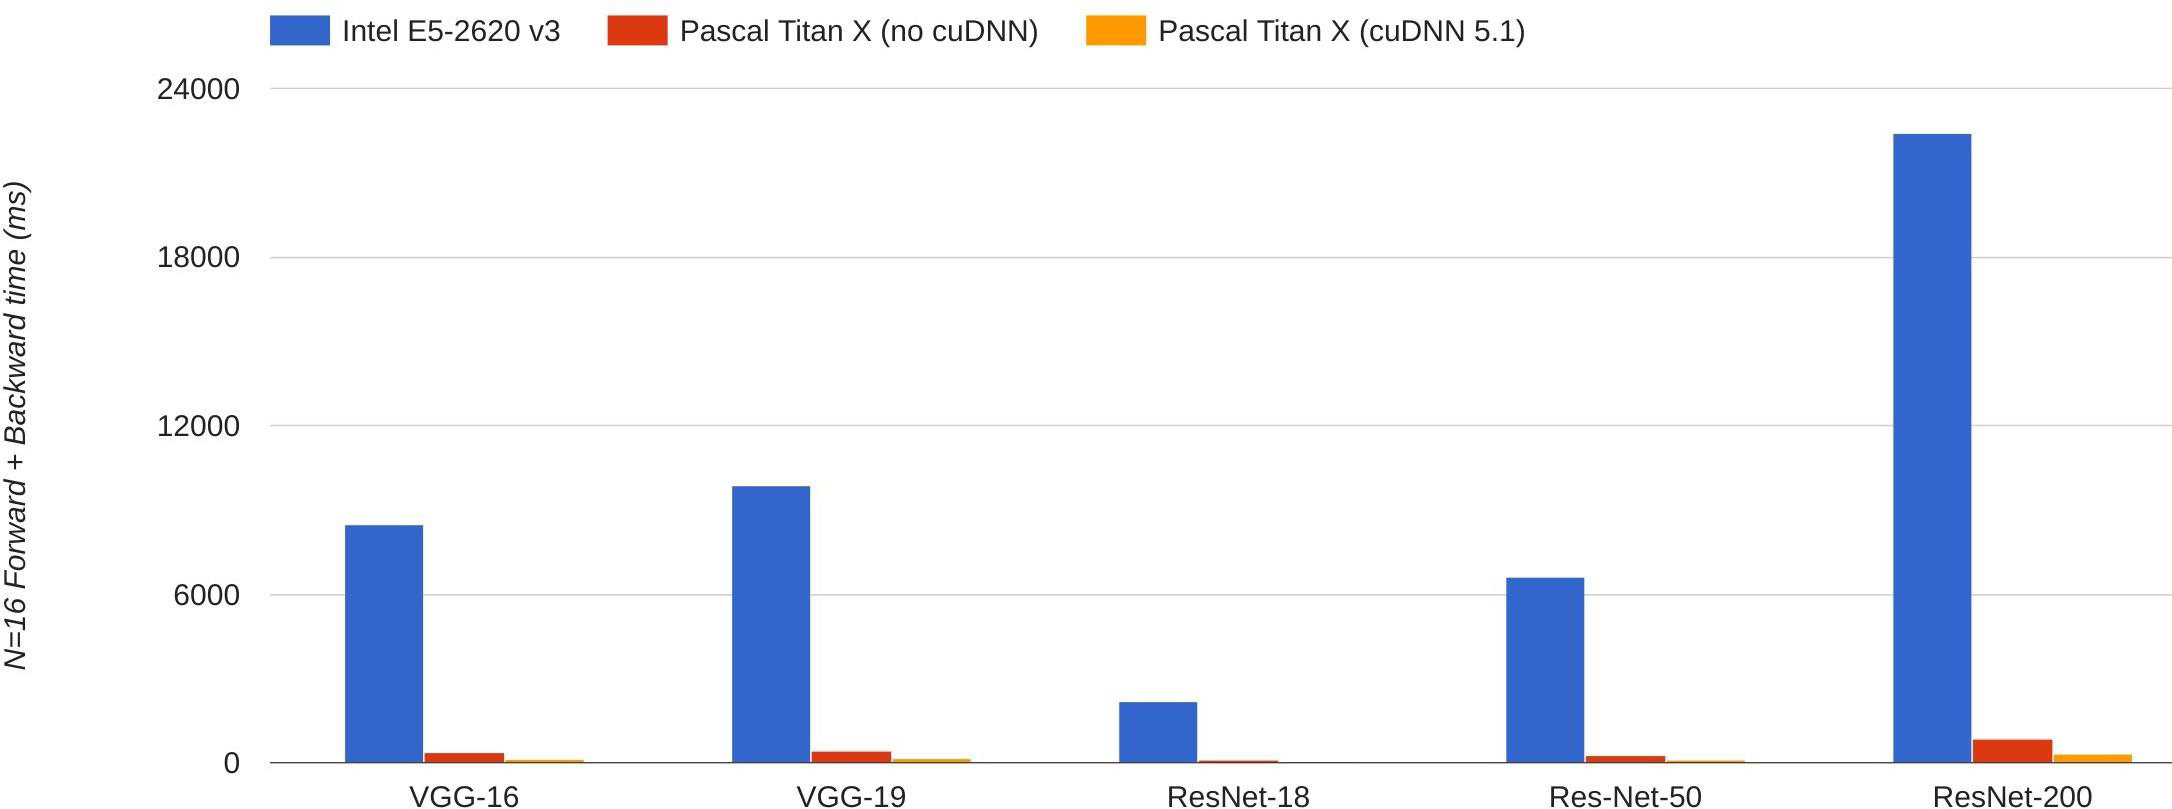
\includegraphics[width=0.9\linewidth]{images/dl-gpus2}
        \caption[CPU vs GPU in practice]{CPU vs GPU in practice (note that CPU performance are not well optimized, so the plot might be a little unfair)}
        \label{fig:dl-gpus2}
    \end{figure}
\end{minipage}

Since data typically resides on disk, training can bottleneck on reading data and transferring to GPU. Possible solutions are:
\begin{myitem}
    \item Read all data into RAM;
    \item Use SSD instead of HDD;
    \item Use multiple CPU threads to prefetch data.
\end{myitem}


\subsection{PyTorch}\label{sec:dl-pytorch}

The main advantages of deep learning frameworks are:
\begin{myitem}
    \item Quick to develop and test new ideas;
    \item Automatically compute gradients;
    \item Run it all efficiently on GPU (wrap cuDNN, etc).
\end{myitem}

PyThorch, in particular, allows to build \textbf{dynamic computation graphs}:
\begin{myitem}
    \item Operations on \textit{Tensors} with \code{requires_grad=True} cause PyTorch to build a computational graph and to perform the actual computations;
    \item \code{loss.backward()} causes search for path between loss and weights (for backpropagation) and perform computation;
    \item On every iteration the graph and the backpropagation path are thrown away, and are rebuild from scratch;
    \item Its's inefficient if we are building the same graph over and over again, but allows to generate different graphs on each iteration under different conditions;
    \item Particularly useful for \textit{recurrent networks}, \textit{recursive networks}, \textit{modular networks}.
\end{myitem}

To overcome the inefficiency of dynamic graphs, if there is no need to change the graph at runtime, one can use \textbf{static computation graphs}:
\begin{myitem}
    \item Build computational graph describing the computation and finding paths for backpropagation;
    \item Reuse the same graph on every iteration;
    \item The framework can optimize the graph before it runs;
    \item Once graph is built, it can be serialized, exported to ONXX, and executed without the code that built it.
\end{myitem}

